\documentclass[11pt,a4paper]{article}

\usepackage[margin=1in]{geometry}
\usepackage[T1]{fontenc}
\usepackage[utf8]{inputenc}
\usepackage{lmodern}
\usepackage{microtype}
\usepackage{booktabs}
\usepackage{tabularx}
\usepackage{array}
\usepackage{xcolor}
\usepackage{hyperref}
\usepackage{enumitem}
\usepackage{listings}
\usepackage{tikz}
\usetikzlibrary{arrows.meta, positioning, shapes.geometric, shapes.multipart, fit, calc}

\hypersetup{
  colorlinks=true,
  linkcolor=blue!55!black,
  urlcolor=blue!55!black,
  citecolor=blue!55!black
}

\setlist[itemize]{topsep=3pt,itemsep=2pt}
\setlist[enumerate]{topsep=3pt,itemsep=2pt}
\renewcommand{\arraystretch}{1.18}

\definecolor{codebg}{RGB}{248,248,248}
\definecolor{codeframe}{RGB}{220,220,220}
\lstdefinestyle{reportcode}{
  backgroundcolor=\color{codebg},
  basicstyle=\ttfamily\small,
  breaklines=true,
  frame=single,
  rulecolor=\color{codeframe},
  columns=fullflexible,
  keepspaces=true,
  showstringspaces=false
}
\lstset{style=reportcode}

\newcolumntype{Y}{>{\raggedright\arraybackslash}X}
\newcommand{\code}[1]{\texttt{#1}}

\title{\textbf{Self-Healing Network Operator for Kubernetes}\\
\large Pod-to-Pod Data Plane Connectivity Through Synthetic Probing}
\author{Computer Networks Course Project}
\date{\today}

\begin{document}
\maketitle

\begin{abstract}
Kubernetes is good at checking whether a container is running, but it does not continuously check whether one pod can reach another pod across the cluster network. This difference matters. A pod can be marked \code{Running} and \code{Ready}, while traffic from that pod to another node is silently dropped because of a CNI issue, a firewall rule, packet loss, or a broad \code{NetworkPolicy}.

This project builds a Kubernetes operator that measures pod-to-pod connectivity from multiple nodes. It deploys one lightweight probe agent on each node, asks these agents to probe each other, builds a directed reachability matrix, classifies the shape of failures, exposes the result through a Kubernetes custom resource, and records measurements for evaluation.

The main contribution is not only detecting that the network is unhealthy. The system also tries to explain where the failure is likely located, such as a node egress problem, node ingress problem, isolated node, pair-specific failure, policy-related failure, or wider cluster partition.
\end{abstract}

\tableofcontents
\newpage

\section{Introduction}

A Kubernetes cluster runs applications inside pods. These pods may be scheduled on different nodes. For a distributed application to work correctly, pods must be able to communicate over the cluster network. This is often called east-west traffic, meaning traffic between workloads inside the cluster.

Kubernetes already has health checks such as liveness probes and readiness probes. These checks answer questions like: ``Is this container alive?'' and ``Should this pod receive service traffic?'' They are useful, but they do not answer a different question: ``Can pod A on node 1 reach pod B on node 2?''

That missing question is the problem this project studies. The cluster may look healthy from the Kubernetes control plane, but the data plane may be broken. The data plane is the actual traffic path used by application packets. If that path fails silently, users see timeouts before the platform reports a clear cause.

\section{Problem Statement}

The project addresses silent pod-to-pod connectivity failures in Kubernetes. A silent connectivity failure is a situation where pods and nodes appear healthy, but traffic between some pods fails or becomes degraded.

Examples include:

\begin{itemize}
  \item a node cannot send traffic to other nodes;
  \item other nodes cannot send traffic to one node;
  \item one pair of nodes has a local connectivity issue;
  \item a node becomes isolated in both directions;
  \item a policy or firewall blocks traffic broadly;
  \item packets are partially lost, causing higher delay, jitter, or unstable throughput.
\end{itemize}

The project asks the following question:

\begin{quote}
Can we continuously measure pod-to-pod connectivity, detect failures quickly, and classify the likely failure location using a simple and robust operator design?
\end{quote}

\section{Objectives}

The project objectives are:

\begin{enumerate}
  \item Build a reproducible multi-node Kubernetes test environment.
  \item Deploy one probe agent per node without bypassing the pod network.
  \item Collect a directed source-to-destination connectivity matrix.
  \item Classify common failure patterns from the matrix.
  \item Expose the current network health as Kubernetes status and Prometheus-style metrics.
  \item Provide fault injection and evaluation scripts.
  \item Measure non-functional requirements: performance, simplicity, and robustness.
\end{enumerate}

The professor's additional non-functional requirements are handled as shown in Table~\ref{tab:nfr}.

\begin{table}[h]
\centering
\caption{Non-functional requirements and project measurements}
\label{tab:nfr}
\begin{tabularx}{\textwidth}{@{}lY@{}}
\toprule
\textbf{Requirement} & \textbf{What the project measures} \\
\midrule
Performance & Detection latency, probe RTT, round duration, throughput estimate \\
Simplicity & Probe count, bytes sent, small fixed components, bounded concurrency \\
Robustness & Loss rate, burst loss, jitter, agent health, safe handling of unknown states \\
\bottomrule
\end{tabularx}
\end{table}

\section{Background}

\subsection{Kubernetes Health Checks}

Kubernetes checks container health mainly through probes configured on pods. A liveness probe can restart a container if it stops responding. A readiness probe can remove a pod from service load balancing if it is not ready. These checks are local to the pod or node.

They do not continuously test every network path between pods. Therefore, a pod may be ready from Kubernetes' point of view but unreachable from another node.

\subsection{Data Plane and Control Plane}

The Kubernetes control plane stores desired state and cluster objects. The data plane is the actual traffic path used when one pod sends packets to another pod. This project focuses on data plane health.

The distinction is important. If the operator itself sends all probes from one central pod, then the system only tests the network from that one source. It cannot detect asymmetric faults, where node A can reach node B but node B cannot reach node A. To avoid this, the project uses distributed agents.

\subsection{Related Tools}

Existing tools solve parts of this problem, but not the full problem addressed here.

\begin{table}[h]
\centering
\caption{Related tools and their limitations for this project}
\begin{tabularx}{\textwidth}{@{}lYY@{}}
\toprule
\textbf{Tool or mechanism} & \textbf{What it does} & \textbf{Limitation for this project} \\
\midrule
Kubernetes liveness/readiness probes & Check whether a container responds & Do not test pod-to-pod paths across nodes \\
Node conditions & Report node-level health & Do not show which pod-to-pod paths fail \\
Goldpinger & Runs as a Kubernetes DaemonSet, tests connectivity between its instances, shows a graph, and exposes Prometheus metrics & Solves detection and visibility well, but does not provide this project's CRD status model, matrix-based failure localization, remediation guardrails, or evaluation workflow \\
Prometheus blackbox exporter & Runs synthetic probes & Usually probes from one location unless many targets are manually configured \\
Service mesh telemetry & Observes real application traffic & Passive; idle paths may stay untested \\
\bottomrule
\end{tabularx}
\end{table}

Goldpinger is the closest open-source baseline for this project.\footnote{\url{https://github.com/bloomberg/goldpinger}} It tackles the same broad problem up to connectivity detection: it answers whether different parts of the cluster can reach each other and makes that information visible. Our project keeps that useful active-probing idea, but adds a few layers on top. It stores the result as Kubernetes custom resource status, classifies the shape of the failure, reports richer non-functional measurements, and includes a repeatable evaluation workflow. In short, Goldpinger tells us that connectivity is broken; this project also tries to say what kind of break it is and how it behaves over time.

This project therefore combines active probing, a Kubernetes custom resource, classification, and evaluation scripts in one small system.

\section{System Overview}

The system has four main runtime pieces:

\begin{enumerate}
  \item a \code{NetworkHealthCheck} custom resource that defines what to measure;
  \item a manager/operator that runs the control loop;
  \item a DaemonSet of agents, one per node;
  \item fault injection and evaluation scripts used during experiments.
\end{enumerate}

The operator does not directly send data plane probes. Instead, it asks each source agent to probe a destination agent. This keeps the measured path close to the real pod network path.

\begin{figure}[h]
\centering
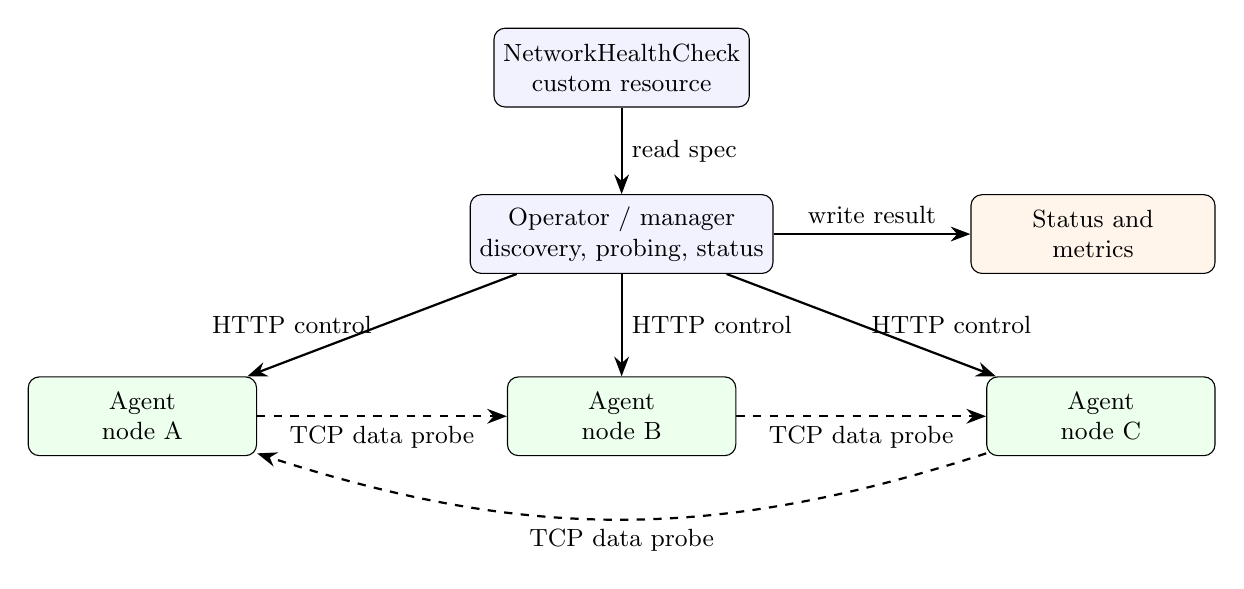
\begin{tikzpicture}[
  font=\small,
  box/.style={draw, rounded corners, align=center, minimum width=3.1cm, minimum height=1.0cm, fill=blue!5},
  agent/.style={draw, rounded corners, align=center, minimum width=2.9cm, minimum height=1.0cm, fill=green!7},
  arrow/.style={-{Stealth[length=2.5mm]}, thick}
]
  \node[box] (crd) {NetworkHealthCheck\\custom resource};
  \node[box, below=1.1cm of crd] (operator) {Operator / manager\\discovery, probing, status};
  \node[agent, below left=1.3cm and 2.7cm of operator] (a1) {Agent\\node A};
  \node[agent, below=1.3cm of operator] (a2) {Agent\\node B};
  \node[agent, below right=1.3cm and 2.7cm of operator] (a3) {Agent\\node C};
  \node[box, right=2.5cm of operator, fill=orange!8] (metrics) {Status and\\metrics};

  \draw[arrow] (crd) -- node[right] {read spec} (operator);
  \draw[arrow] (operator) -- node[above] {write result} (metrics);
  \draw[arrow] (operator) -- node[left] {HTTP control} (a1);
  \draw[arrow] (operator) -- node[right] {HTTP control} (a2);
  \draw[arrow] (operator) -- node[right] {HTTP control} (a3);
  \draw[arrow, dashed] (a1) -- node[below] {TCP data probe} (a2);
  \draw[arrow, dashed] (a2) -- node[below] {TCP data probe} (a3);
  \draw[arrow, dashed] (a3) to[bend left=18] node[below] {TCP data probe} (a1);
\end{tikzpicture}
\caption{High-level architecture. The operator controls the experiment, while agents send the actual data-plane probes.}
\label{fig:architecture}
\end{figure}

The result is stored as a matrix. A directed matrix means \code{node-a -> node-b} and \code{node-b -> node-a} are separate entries. This is necessary because network failures can be one-way.

\begin{figure}[h]
\centering
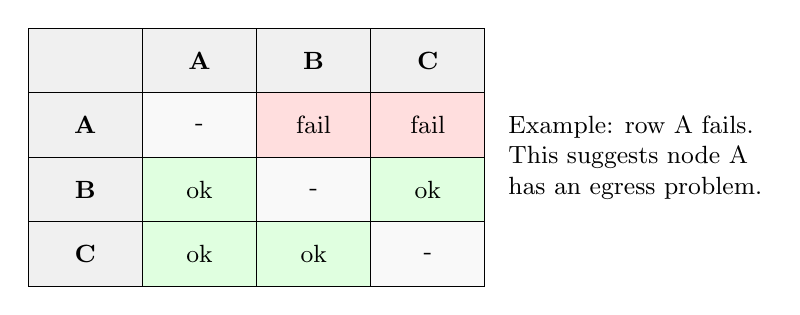
\begin{tikzpicture}[
  font=\small,
  cell/.style={draw, minimum width=1.45cm, minimum height=0.82cm, align=center},
  good/.style={cell, fill=green!12},
  bad/.style={cell, fill=red!13},
  header/.style={cell, fill=gray!12, font=\small\bfseries}
]
  \node[header] at (0,0) {};
  \node[header] at (1.45,0) {A};
  \node[header] at (2.90,0) {B};
  \node[header] at (4.35,0) {C};
  \node[header] at (0,-0.82) {A};
  \node[header] at (0,-1.64) {B};
  \node[header] at (0,-2.46) {C};
  \node[cell, fill=gray!5] at (1.45,-0.82) {-};
  \node[bad] at (2.90,-0.82) {fail};
  \node[bad] at (4.35,-0.82) {fail};
  \node[good] at (1.45,-1.64) {ok};
  \node[cell, fill=gray!5] at (2.90,-1.64) {-};
  \node[good] at (4.35,-1.64) {ok};
  \node[good] at (1.45,-2.46) {ok};
  \node[good] at (2.90,-2.46) {ok};
  \node[cell, fill=gray!5] at (4.35,-2.46) {-};
  \node[align=left, right=0.9cm of {$(4.35,-1.23)$}] {Example: row A fails.\\This suggests node A\\has an egress problem.};
\end{tikzpicture}
\caption{Directed matrix intuition. A failed row points to an outgoing traffic problem from that source.}
\label{fig:matrix}
\end{figure}

\section{Platform and Deployment}

The platform layer provides the environment in which the rest of the project runs. The repository uses KIND to create a local multi-node Kubernetes cluster. KIND is useful for this project because each Kubernetes node is a Docker container. That makes fault injection repeatable through commands such as \code{iptables} and \code{tc netem}.

The cluster configuration is stored in \code{hack/kind-cluster.yaml}. The project uses one control-plane node and three worker nodes. Calico is used as the CNI plugin, and the default KIND CNI is disabled. This gives a real pod network and supports the network policy scenarios used later.

\begin{table}[h]
\centering
\caption{Platform files}
\begin{tabularx}{\textwidth}{@{}lY@{}}
\toprule
\textbf{File} & \textbf{Purpose} \\
\midrule
\code{hack/setup-cluster.sh} & Creates the KIND cluster and installs Calico \\
\code{hack/reset-cluster.sh} & Tears down the local cluster \\
\code{Dockerfile} & Builds the manager image \\
\code{Dockerfile.agent} & Builds the agent image \\
\code{config/namespace.yaml} & Creates the \code{netprobe-system} namespace \\
\code{config/kustomization.yaml} & Applies all Kubernetes manifests together \\
\code{Makefile} & Provides common build, deploy, test, and evaluation commands \\
\bottomrule
\end{tabularx}
\end{table}

The \code{Makefile} keeps project operation simple. For example, \code{make cluster-up} creates the cluster, \code{make images} builds images, \code{make load} loads them into KIND, and \code{make deploy} applies the Kubernetes manifests.

\section{Distributed Probe Agent}

The distributed probe agent runs on every node. The agent is deployed as a DaemonSet, which means Kubernetes schedules one copy on each node. The manifest is in \path{config/agent/daemonset.yaml}.

Each agent exposes two ports.

\begin{table}[h]
\centering
\caption{Agent ports}
\begin{tabularx}{0.72\textwidth}{@{}lY@{}}
\toprule
\textbf{Port} & \textbf{Purpose} \\
\midrule
\code{8080} & Control API used by the operator \\
\code{9376} & Data-plane TCP listener used as the probe target \\
\bottomrule
\end{tabularx}
\end{table}

Keeping these ports separate is an important design choice. The control API tells the agent what to do. The data port is the actual network path being tested. If both used the same port, it would be harder to tell whether the control path failed or the data path failed.

The agent exposes the endpoints in Table~\ref{tab:agent-endpoints}.

\begin{table}[h]
\centering
\caption{Agent endpoints}
\label{tab:agent-endpoints}
\begin{tabularx}{0.82\textwidth}{@{}lY@{}}
\toprule
\textbf{Endpoint} & \textbf{Meaning} \\
\midrule
\code{/healthz} & Reports that the agent is running and includes node/pod identity \\
\code{/probe} & Runs a probe to a requested target and returns JSON \\
\code{/metrics} & Reports a simple agent health metric \\
\bottomrule
\end{tabularx}
\end{table}

The probe endpoint accepts parameters such as target address, timeout, count, and payload size. During a probe round, the agent tries several TCP connections and writes a small payload. It then reports success, loss rate, RTT, jitter, burst loss, bytes sent, throughput estimate, and probe counts.

This means the agent supports both functional measurement and non-functional measurement. Functional measurement answers ``can it connect?'' Non-functional measurement answers ``how well did it connect?''

\section{Operator and Kubernetes API}

The operator implements the control logic. It periodically reads \code{NetworkHealthCheck} resources, discovers running agent pods, asks agents to probe each other, stores the matrix, and writes status back to Kubernetes.

The custom resource definition is in \code{config/crd/networkhealthcheck-crd.yaml}. A sample object is in \code{config/samples/networkhealthcheck-sample.yaml}.

\begin{lstlisting}[caption={Sample NetworkHealthCheck specification}]
apiVersion: network.selfheal.io/v1alpha1
kind: NetworkHealthCheck
metadata:
  name: cluster-mesh
spec:
  interval: "15s"
  probeTimeout: "2s"
  probeType: TCP
  probeCount: 5
  probePayloadBytes: 1024
  topology: FullMesh
  sampleDegree: 3
  failureThreshold: 3
  successThreshold: 2
  maxConcurrentProbes: 64
  remediation:
    enabled: true
    dryRun: false
\end{lstlisting}

The controller performs these steps:

\begin{enumerate}
  \item List the agent pods with label \code{app=netprobe-agent}.
  \item Ignore pods that are not running or do not have a pod IP.
  \item Build directed probe pairs between the discovered agents.
  \item Run probes with bounded concurrency.
  \item Build a matrix keyed by \code{sourceNode->destinationNode}.
  \item Pass the matrix to the analysis package.
  \item Write the classification and reachability entries into resource status.
  \item Store the latest values for Prometheus-style metrics.
  \item Optionally create a remediation plan, depending on configuration.
\end{enumerate}

The status fields are shown in Table~\ref{tab:status}.

\begin{table}[h]
\centering
\caption{Important status fields}
\label{tab:status}
\begin{tabularx}{\textwidth}{@{}lY@{}}
\toprule
\textbf{Status field} & \textbf{Meaning} \\
\midrule
\code{observedGeneration} & Version of the spec that was observed \\
\code{lastProbeTime} & Time when the latest probe round was stored \\
\code{classification} & Current classifier result \\
\code{classificationConfidence} & Confidence score from the classifier \\
\code{suspectNodes} & Nodes related to the suspected fault \\
\code{reachability} & Directed probe matrix with metrics \\
\code{conditions} & Kubernetes-style health condition \\
\bottomrule
\end{tabularx}
\end{table}

The controller preserves \code{lastTransitionTime} when the condition has not actually changed. This is important for evaluation because detection latency depends on the time when the system first moved from healthy to unhealthy.

\section{Analysis and Failure Classification}

The analysis layer takes the directed matrix and returns a verdict.

The classifier is implemented in \code{pkg/analysis/classifier.go}. It is designed to be simple enough to explain and test. It does not need machine learning. It uses the shape of failures in the matrix.

For example, imagine three nodes: A, B, and C. If A cannot reach B or C, but B and C can still reach A, then A likely has an egress problem. In matrix form, the row for A fails. If B and C cannot reach A, but A can reach them, then A likely has an ingress problem. In matrix form, the column for A fails.

\begin{figure}[h]
\centering
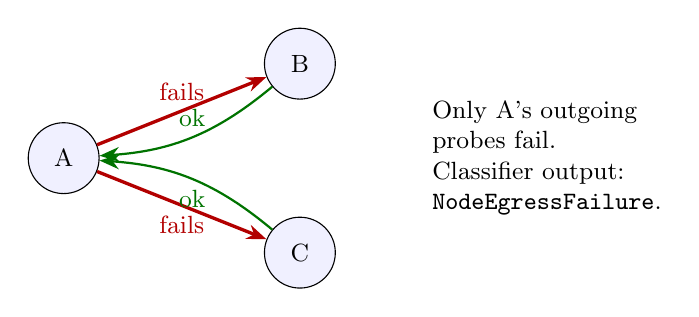
\begin{tikzpicture}[
  font=\small,
  node/.style={circle, draw, minimum size=9mm, fill=blue!6},
  badarrow/.style={-{Stealth[length=2.5mm]}, very thick, red!70!black},
  goodarrow/.style={-{Stealth[length=2.5mm]}, thick, green!45!black}
]
  \node[node] (a) at (0,1.6) {A};
  \node[node] (b) at (3.0,2.8) {B};
  \node[node] (c) at (3.0,0.4) {C};
  \draw[badarrow] (a) -- node[above] {fails} (b);
  \draw[badarrow] (a) -- node[below] {fails} (c);
  \draw[goodarrow, bend left=18] (b) to node[above] {ok} (a);
  \draw[goodarrow, bend right=18] (c) to node[below] {ok} (a);
  \node[align=left, right=1.1cm of b, yshift=-1.2cm] {Only A's outgoing\\probes fail.\\Classifier output:\\\code{NodeEgressFailure}.};
\end{tikzpicture}
\caption{Classifier example for a node egress failure.}
\label{fig:classifier}
\end{figure}

\begin{table}[h]
\centering
\caption{Classifier rules}
\begin{tabularx}{\textwidth}{@{}YY@{}}
\toprule
\textbf{Matrix pattern} & \textbf{Classification} \\
\midrule
No failed pairs & \code{Healthy} \\
One directed pair fails & \code{PairLocalFailure} \\
All outgoing probes from one node fail & \code{NodeEgressFailure} \\
All incoming probes to one node fail & \code{NodeIngressFailure} \\
All incoming and outgoing probes for one node fail & \code{NodeIsolated} \\
Most or all pairs fail across the cluster & \code{ClusterPartition} \\
All pairs fail with connection refused & \code{PolicyScopedFailure} \\
Agent/control error or unclear pattern & \code{Unknown} \\
\bottomrule
\end{tabularx}
\end{table}

The \code{Unknown} class is important. It prevents the system from making a confident claim when the evidence is not clear. This is especially important if remediation is enabled.

The analysis package also contains a hysteresis tracker. Hysteresis means that the system can wait for repeated failures before marking a pair degraded, and can wait for repeated successes before marking it recovered. This reduces noise from short transient events. In the current codebase, this tracker exists as a tested analysis component, while the live controller path calls the stateless \code{Evaluate} entry point directly.

\section{Remediation Safety}

The project includes a remediation planning path in \code{internal/controller/remediation.go}. Remediation is intentionally conservative.

The planner refuses to act when:

\begin{itemize}
  \item the verdict is \code{Healthy};
  \item the verdict is \code{Unknown};
  \item the confidence score is below \code{0.8};
  \item the action would be unsafe for broad failures such as cluster partition or policy-scoped failure.
\end{itemize}

For node-related failures, the implemented action can restart the matching agent pod. This is a cautious remediation stub rather than a full network repair system. It shows how remediation can be wired while preserving safety guardrails.

\section{Monitoring and Observability}

The manager exposes \code{/metrics}. The current implementation writes Prometheus-style text metrics based on the latest probe round. Important metrics are listed in Table~\ref{tab:metrics}.

\begin{table}[h]
\centering
\caption{Prometheus-style metrics}
\label{tab:metrics}
\begin{tabularx}{\textwidth}{@{}lY@{}}
\toprule
\textbf{Metric} & \textbf{Meaning} \\
\midrule
\code{netprobe\_manager\_up} & Manager process is running \\
\code{netprobe\_pair\_reachable} & Whether a directed pair was reachable \\
\code{netprobe\_pair\_rtt\_seconds} & Average pair latency \\
\code{netprobe\_pair\_jitter\_seconds} & Pair jitter \\
\code{netprobe\_pair\_loss\_rate} & Pair loss rate \\
\code{netprobe\_pair\_loss\_burst} & Maximum consecutive failed probes \\
\code{netprobe\_pair\_throughput\_bytes\_per\_second} & Synthetic throughput estimate \\
\code{netprobe\_pair\_bytes\_sent} & Bytes sent in latest pair round \\
\code{netprobe\_pair\_probes\_sent} & Probe attempts in latest pair round \\
\code{netprobe\_round\_duration\_seconds} & Wall-clock duration of the latest round \\
\code{netprobe\_mesh\_health} & Whether the latest verdict is healthy \\
\code{netprobe\_classification} & Latest classification confidence \\
\bottomrule
\end{tabularx}
\end{table}

The project also includes monitoring manifests under \code{config/monitoring/}, including a ServiceMonitor and Grafana dashboard configuration.

\section{Fault Injection}

To test detection and classification, the project uses controlled fault scenarios. These are implemented in \code{hack/inject-fault.sh}.

\begin{table}[h]
\centering
\caption{Fault scenarios}
\begin{tabularx}{\textwidth}{@{}lYY@{}}
\toprule
\textbf{Scenario} & \textbf{Fault} & \textbf{Expected classification} \\
\midrule
F1 & Healthy baseline & \code{Healthy} \\
F2 & Block inbound traffic on the target agent data port & \code{NodeIngressFailure} \\
F3 & Block outbound traffic from the target agent data port & \code{NodeEgressFailure} \\
F4 & Kill Calico node pod and isolate the agent data port & \code{NodeIsolated} \\
F5 & Add 40 percent packet loss with \code{tc netem} & \code{Degraded} or degraded evidence in metrics \\
F6 & Apply deny-all \code{NetworkPolicy} & \code{ClusterPartition} or \code{PolicyScopedFailure}, depending on observed error pattern \\
\bottomrule
\end{tabularx}
\end{table}

These scenarios allow the project to test both complete failures and degraded behavior. Complete failures mainly affect classification. Partial packet loss is especially useful for robustness metrics such as loss rate, jitter, and burst loss.

\section{Evaluation Methodology}

The evaluation layer measures the system using repeatable experiments. The key script is \code{hack/measure-mttd.sh}. It clears previous faults, injects a chosen scenario, records the injection timestamp, polls the \code{NetworkHealthCheck} status, and writes a CSV row when an unhealthy transition is observed.

The evaluation uses the scenarios listed in Table~\ref{tab:p5-scenarios}. These scenarios were selected because each one creates a different shape in the directed reachability matrix. This is important because the classifier does not simply count failures. It looks at where the failures appear: in one row, in one column, around one node, across the whole cluster, or as partial loss.

\begin{table}[h]
\centering
\caption{Specific scenarios used in evaluation}
\label{tab:p5-scenarios}
\scriptsize
\begin{tabularx}{\textwidth}{@{}lYYYY@{}}
\toprule
\textbf{Scenario} & \textbf{Injected condition} & \textbf{Why it is included} & \textbf{Expected classifier result} & \textbf{Important measurements} \\
\midrule
F1 & Healthy baseline; no fault is applied. & Establishes the normal matrix before fault trials and checks that the system does not report a failure when the cluster is healthy. & \code{Healthy} & RTT, jitter, throughput, bytes per round, and probe count under normal conditions. \\
F2 & Inbound TCP traffic to the target agent's data port \code{9376} is blocked inside the agent pod on the selected node. & Creates a column-shaped failure: other nodes cannot reach the selected node, but the selected node may still reach others. & \code{NodeIngressFailure} & MTTD, classification accuracy, failed incoming pairs, loss rate, and burst loss. \\
F3 & Outbound TCP traffic from the target agent to data port \code{9376} is blocked inside the agent pod on the selected node. & Creates a row-shaped failure: the selected node cannot reach other nodes, but other nodes may still reach it. & \code{NodeEgressFailure} & MTTD, classification accuracy, failed outgoing pairs, loss rate, and burst loss. \\
F4 & The Calico node pod on the selected worker is deleted, and the agent data path is blocked in both directions for that node. & Represents a node-level network isolation case where both incoming and outgoing data-plane paths fail. & \code{NodeIsolated} & MTTD, suspect node correctness, bidirectional loss, and recovery behavior after clearing. \\
F5 & A \code{tc netem} rule adds 40 percent packet loss on the selected KIND worker. & Tests degradation rather than a complete partition. This is the main scenario for robustness metrics. & Degraded evidence in status and metrics; classification may remain \code{Healthy} if some probes still succeed. & Loss rate, burst loss, jitter, RTT change, and throughput drop. \\
F6 & A deny-all \code{NetworkPolicy} is applied in the agent namespace. & Creates a broad policy-caused communication failure across the mesh. & \code{ClusterPartition} or \code{PolicyScopedFailure}, depending on the observed connection error pattern. & MTTD, broad failure rate, classifier result, and confidence. \\
\bottomrule
\end{tabularx}
\end{table}

For the main evaluation run, F2 through F6 are repeated because they are actual injected faults. F1 is used as the healthy starting point and cleanup baseline before each trial. This keeps each trial independent from the previous one.

The full sweep is run with:

\begin{lstlisting}[language=bash]
TRIALS=10 ./hack/run-p5-evaluation.sh
\end{lstlisting}

A shorter run can be used during demonstrations:

\begin{lstlisting}[language=bash]
TRIALS=1 SCENARIOS="F2 F3 F5" ./hack/run-p5-evaluation.sh
\end{lstlisting}

The raw output is stored in \code{docs/results/mttd-results.csv}. The summary script \code{hack/summarize-results.py} produces \code{docs/results/p5-summary.md}.

\subsection{Evaluation Metrics}

\begin{table}[h]
\centering
\caption{CSV columns produced by the evaluation scripts}
\begin{tabularx}{\textwidth}{@{}lY@{}}
\toprule
\textbf{Column} & \textbf{Meaning} \\
\midrule
\code{scenario} & Fault scenario ID \\
\code{trial} & Trial number \\
\code{inject\_ts} & Fault injection time \\
\code{detect\_ts} & Time when unhealthy status was detected \\
\code{mttd\_ms} & Detection latency in milliseconds \\
\code{predicted\_class} & Classifier output \\
\code{true\_class} & Expected class for the injected fault \\
\code{confidence} & Classifier confidence \\
\code{avg\_rtt\_ms} & Average RTT across matrix entries \\
\code{avg\_jitter\_ms} & Average jitter across matrix entries \\
\code{avg\_loss\_rate} & Average loss rate across matrix entries \\
\code{max\_burst\_loss} & Worst burst loss observed \\
\code{avg\_throughput\_bps} & Average synthetic throughput \\
\code{total\_bytes\_sent} & Bytes sent in the round \\
\code{probe\_count} & Total attempted probes \\
\bottomrule
\end{tabularx}
\end{table}

\subsection{Performance}

Performance is measured in two ways. First, detection latency measures how long the system takes to move from injected fault to unhealthy status. Second, probe-level performance measures RTT, round duration, and throughput estimate.

This separation is useful because a system may have fast probes but slow detection if the interval is large, or it may have quick detection but expensive probe rounds if too many pairs are measured.

\subsection{Simplicity}

Simplicity is measured through design and operational cost. The system has one manager deployment and one agent per node. The probe protocol is HTTP plus TCP. The matrix format is a simple map from \code{source->destination} to a result object.

The measured simplicity indicators are probe count, bytes per round, and the fixed number of deployed components. These are easy to explain and easy to compare across cluster sizes.

\subsection{Robustness}

Robustness means the system should keep giving useful information even when the network is unstable. The project measures this using loss rate, burst loss, jitter, and control-channel errors.

The classifier treats agent control errors as \code{Unknown} instead of pretending they are data plane failures. This is a robustness feature because it avoids false certainty when the measurement system itself may be impaired.

\section{Testing}

The repository includes tests for major pure-code components:

\begin{itemize}
  \item controller agent discovery;
  \item probe round matrix construction;
  \item bounded concurrency;
  \item status updates and conflict retry;
  \item preserving transition time for stable MTTD;
  \item classifier behavior over fixture matrices;
  \item ambiguous cases that should return \code{Unknown};
  \item agent/control errors;
  \item hysteresis state transitions;
  \item remediation planning safety.
\end{itemize}

The fixture files in \code{contracts/fixtures/} describe expected matrix shapes for healthy, degraded, isolated, ingress, egress, pair-local, ambiguous, and policy-scoped cases.

\section{Measured Results}

The evaluation was run on the KIND-based test cluster with three trials for each injected fault scenario from F2 to F6. F1 was used as the healthy baseline and cleanup state before each trial, so it is not shown as a fault row. The results are shown in Table~\ref{tab:results}.

During the run, F4 printed Kubernetes warnings because the script intentionally uses forced deletion of the Calico pod to create a node/CNI disruption. F5 timed out in all three trials, so it never returned a detected unhealthy transition within the 120 second polling window. Because of that, the detection-row averages such as RTT, jitter, loss, burst loss, and throughput are not applicable for F5 in this table. The F6 cleanup printed \code{NotFound} messages when the deny-all policy was already absent; this is an idempotent cleanup message and did not prevent the F6 trials from running.

\begin{table}[h]
\centering
\caption{Measured evaluation results}
\label{tab:results}
\scriptsize
\begin{tabularx}{\textwidth}{@{}lYYYYYYYYY@{}}
\toprule
\textbf{Scenario} & \textbf{Trials} & \textbf{Acc.} & \textbf{MTTD ms} & \textbf{RTT ms} & \textbf{Jitter ms} & \textbf{Loss rate} & \textbf{Max burst} & \textbf{B/s} & \textbf{Probes} \\
\midrule
F2 & 3 & 1.00 & 15073.0 & 0.396 & 0.073 & 0.333 & 5 & 1.157e6 & 30.0 \\
F3 & 3 & 1.00 & 12991.7 & 0.416 & 0.097 & 0.333 & 5 & 1.101e6 & 30.0 \\
F4 & 3 & 1.00 & 18614.7 & 0.194 & 0.039 & 0.667 & 5 & 5.858e5 & 30.0 \\
F5 & 3 & 0.00 & timeout & n/a & n/a & n/a & n/a & n/a & n/a \\
F6 & 3 & 1.00 & 14745.7 & 0.000 & 0.000 & 1.000 & 5 & 0.00 & 30.0 \\
\bottomrule
\end{tabularx}
\end{table}

The complete-failure scenarios were detected reliably. F2, F3, F4, and F6 all reached the expected classification in every completed trial. F2 and F3 had one-third average loss because one row or one column of the directed matrix failed. F4 had two-thirds average loss because the selected node was isolated in both directions. F6 had complete loss and zero throughput because the deny-all policy blocked the mesh-wide data path.

The F5 timeout is also informative. Since the experiment did not reach a detected unhealthy state, there was no completed detection row from which to report the corresponding RTT, jitter, loss, burst-loss, or throughput averages. Those cells are therefore marked as not applicable rather than measured values.

\section{Limitations}

The project has several important limitations.

First, KIND runs nodes as containers on a single host. This is excellent for reproducible testing, but it is not the same as measuring real physical machines connected by a real network. The latency and throughput numbers should therefore be treated as local experimental measurements, not as production network benchmarks.

Second, the throughput value is synthetic. The agent writes a small payload over TCP and computes bytes per second for that probe round. This is useful for comparing scenarios inside the same test setup, but it is not a replacement for a dedicated bandwidth tool such as iperf.

Third, the live controller currently builds full directed probe pairs between discovered agents. The CRD contains topology fields such as \code{FullMesh}, \code{Sampled}, and \code{sampleDegree}, but sampled topology is not fully implemented in the live probe planner.

Fourth, the hysteresis tracker exists in the analysis package, but the current live controller uses the stateless classifier entry point directly. This means repeated-round debouncing is available as code but not fully integrated into the live reconciliation path.

Fifth, remediation is intentionally limited. It can plan and perform conservative agent pod restarts for certain node-related cases, but it does not repair arbitrary CNI, policy, or underlay failures.

\section{Future Work}

The most useful next improvements are:

\begin{enumerate}
  \item Integrate hysteresis directly into the live controller loop.
  \item Fully implement sampled topology so large clusters do not require all ordered pairs every round.
  \item Add real Prometheus client library registration instead of manually writing metric text.
  \item Add stronger event handling so Kubernetes Events are emitted only on meaningful transitions.
  \item Add a stronger remediation budget with cooldowns and per-node rate limits.
  \item Add DNS probing because many real incidents are name-resolution failures rather than raw TCP failures.
  \item Run the same evaluation on a larger real cluster to compare with KIND results.
\end{enumerate}

\section{Conclusion}

This project builds a small but complete system for active pod-to-pod network health checking in Kubernetes. The main idea is simple: place an agent on each node, ask agents to probe each other, build a directed matrix, classify the matrix, and publish the result as Kubernetes status and metrics.

The design improves on basic health checks because it measures the actual paths between pods. It also improves on simple dashboards because the result becomes part of Kubernetes state and can be evaluated through repeatable experiments.

The final system covers platform setup, agent implementation, operator control logic, classification, safety-aware remediation planning, and evaluation. It can detect connectivity failures, report where they are likely located, and measure performance and robustness indicators such as latency, throughput, loss, burst loss, and jitter.

\end{document}
